\documentclass[fleqn,10pt]{wlscirep}
\usepackage[utf8]{inputenc}
\usepackage{amsfonts,amssymb,amsmath}
\usepackage{graphicx}


\title{Complexity Insights into Circular Economy}

\author[1]{Joris Broere}
\author[2]{Christine Moore}
\author[3]{Juste Raimbault}
\author[4]{Jesus Mario Serna}
\author[5]{Marius Somveille}
\author[6]{Evelyn Strombom}
\author[7]{Lorraine Sugar}
\author[8]{Ben Zhu}

\affil[1]{Affiliation, department, city, postcode, country}
\affil[2]{Affiliation, department, city, postcode, country}

\affil[*]{corresponding.author@email.example}

\affil[+]{these authors contributed equally to this work}

%\date{July 6, 2016}


%\keywords{Keyword1, Keyword2, Keyword3}


\begin{abstract}

\end{abstract}

\begin{document}


\flushbottom
\maketitle

\thispagestyle{empty}


\section*{General project description: CSSS 2016}
The 'circular economy' is recent approach on questions of sustainability. The current 'take, make, waste' way of producing is considered to be not sustainable anymore. Current thoughts on 'closing the loop' mechanisms on producing and consuming are booming in many different academic fields. However, not yet from an integrated point of view. The idea of 'closing the loop' mechanisms corresponds to complex system paradigms, however complexity science has hardly been utilized in this field. In this project we started brainstorming on how complexity science can contribute to the field of circular economy. We think there are many ways in which complexity science can contribute, both in methods and in theory. 

In the past four weeks at CSSS 2016 we focused by modeling the circular economy by means of an agent based model. So far we have made an toy model that models waste flow between actors on the level of organizations/businesses. The purpose of this model is to investigate how waste flow is affected by different parameters such as, distance, clustering, transportation cost and other parameters. After the CSSS 2016 we will continue to work on the model by making validating it to real work settings. The model will be validated by applying it to real world spatial maps and infrastructures, and calibrate it to data of first implementations of `circular economy practices'. The goal is to make a basis for an open source circular economy application that can be used to monitor the circular economy, as well as create a market place for waste products. In what follows a first draft of the paper of the toy model.



%%%%%%%%%%%%%%%%%%
\section{Introduction}

% model rationale etc

\subsection{Description of circular economy concept}

The notion of a circular economy proposes that traditionally separate industries act collectively to obtain a mutual competitive advantage through their physical exchanges of materials, energy, water, and byproducts~\cite{chertow2000industrial}. Described as a material symbiosis, a circular economy approach seeks to recycle residual waste or by-products through the development of complex interlinkages between companies and firms.  In direct contrast with the conventional linear economic approach of material production of produce-use-dispose, the circular economy concept seeks to reduce the uptake of virgin materials while also reducing total waste production by accommodating the cycle of materials (EU Document). This concept is distinct from traditional recycling whereby products are often reduced to their lowest nutrient level, and then disposed of. In a circular economy approach, waste or by product materials of one firm have the potential to become high nutrient level inputs to another firm. As a result, there isn’t a sequential downgrading of waste or by-products, but rather a full cycling of materials. 


%%%%%%%%%%%%%%%%%%%%%
\subsection{Prospective Literature review}

% could we copy-paste here the literature review that was done in the google doc ?-> would give a bit more background 

\textit{This section gives a broad prospective literature review, not necessarily structured.}

\paragraph{Urban Metabolism}

References on Urban Metabolism : \cite{kennedy2007changing}, \cite{kennedy2011study}, \cite{newcombe1978metabolism}, \cite{bodini2012cities}, \cite{hoornwegmainstreaming}.

\cite{olsen1982urban} give theory of the city as an organism, associated temporal and spatial scales, corresponding cycles, economic variables and human scales. Cycles are detailed, but no numerical application nor conceptual model, stays at the qualitative descriptive level. Can be used in our case as a “theoretical backup” reference.


\paragraph{Industrial Ecology}

\cite{bai2007industrial} is an editorial for journal of Indus. Ecology (close to an opinion paper). Relatively close to our position, as argues that study of cities and industrial ecology have to be reconciled ($\simeq$ look at industrial ecology from a complexity perspective). ``Tackling global problems at the local level.'' is in the spirit of our rationale.


\paragraph{Complexity in industrial symbiosis literature}

\cite{li2015resilience} : this paper does simulations based on real data on the resilience of industrial symbioses networks by looking at what happens if a node get removed.

\cite{zhu2013exploring} : Agent based model on resilience in industrial ecosystems, made in Netlogo.

\cite{may1973stability} : Potential interesting book.



\paragraph{Ecology}


Citation on information theory in ecological systems. Could be interesting for model comparison : \cite{ulanowicz1991ecosystem}




\subsection{Existing studies into circular economies}

This approach has been practically adopted on a small scale in Asia, specifically in China, via the establishment of eco-industrial parks. 

There have been a number of publications which have assessed the theoretical options and implications of adopting a circular economy approach. 

\subsection{Rational for our model/study}

While many large organizations, including the EU and the UN,  have expressed interest in adopting the a circular economy approach, much work which has been done has either focused on small scale applied examples or on theoretical frameworks and models. As such, studies are needed which seek to model the dynamics of the circular economy concept, and begin to offer larger more generalized examples of how the concept feasibly be achieved. 


%%%%%%%%%%%%%%%%%%
\section{Model Description}

%%%%%%%%%%%%%%%%%%
\subsection{Model Core}

\paragraph{Model setup}

The core part of the model is assumed to take place at a single scale, but with variable spatial range. The agents are $N$ companies indexed by $1\leq i\leq N$, that have a fixed spatial position $\vec{x}_i$. In order to focus on the exchange of by-products as inputs for other companies, we choose not to model the effective product nor the ``external'' inputs. For the sake of simplicity, by-products are assumed to be described by a finite-dimensional real variable $\vec{y}\in \mathbb{R}^d$. Finite values are a reasonable domain for by-products characteristics as it allows to normalize along each axis and take $\vec{y} \in \left[0,1\right]^d$. Each company has a demand function and an offer function, which were used to establish links between pairs of companies (i.e. exchange of by-products). These function are defined in a simple manner by $\vec{D}_i (\vec{y})= D_i^{(0)}\cdot \vec{d}_i (\vec{y})$ and $\vec{O}_i (\vec{y})= O_i^{(0)}\cdot \vec{o}_i (\vec{y})$, where $\vec{d}_i$ and $\vec{o}_i$ are multivariate probability densities. We started our simulation with a set of companies that were not linked with each other, and then grew the network based on rules determining exchange of by-products (effectively creating links between companies).



\paragraph{Growing the circular economy network}

The temporal scope of the model evolution was assumed to be at a mesoscopic time scale, following the assumption that companies localization and the surrounding urban environment (which includes the transportation cost landscape) remain constant. The temporal dynamics consist of network growth, i.e. the progressive establishment of complementary links between companies that correspond to flows of by-products.

Two factors were used to establish links between companies (i.e. exchange of by-products): 1) the geographical distance separating them, and 2) the match between demand and offer. The geographical interaction potential ($V_{ij}$; i.e. probability of two companies interacting based on their geographical location) decreased exponentially with distance such as $V_{ij}=\frac{1}{d_{ij}^{\alpha}}$ % we probably need references here %
Increasing geographical distance also meant increasing transportation cost (in a linear fashion). The match between a company's offer (i.e. what it wastes after production) and another company's demand (i.e. what it could use for production) was computed along a "by-product" axis (an abstract by-product one-dimensional space, which could later be generalized to a multi-dimensional space). Along this by-product axis, the offer function and a demand function of each company are represented by a gaussian density distribution. We computed the overlap between pairs of demand and offer functions \(o = \int min(O,D) dx\) – a higher overlap indicating a higher probability that the two companies exchange by-products – and used an overlap threshold $T_o$ above which companies could potentially exchange by-products. This modeling approach was inspired by the ecological literature on probability niche models in complex food webs \cite{williams2000simple,williams2010probabilistic}. In these models, predation interaction between two species was modeled as the probability of species i eating another species j based on their values along a "niche" axis. More specifically, species i has a feeding optimum and the probability of eating species j declines has the niche position of species j gets further from this feeding optimum, which was model using a Gaussian centered on the feeding optimum. 

The utility function associated with each potential exchange of by-products between two companies was defined as follows:
\[u = \frac{o - c*d}{d_{max}}\]
where $o$ is the overlap between the two companies in by-product space, $c$ is the transportation cost, $d$ is the geographical distance between the two companies, and $d_{max}$ is the maximum distance between any two companies in the system.


In our model, at each time step, the following set of rules was applied:
\begin{itemize}
\item A company, the ``current contractor'' is drawn at random % distrib
\item Potential partners are drawn
\begin{itemize}
\item according to geographical interaction potential $V_{ij}=\frac{1}{d_{ij}^{\alpha}}$
\item among these, the ones whose overlap is above $T_o$
% detail the overlap in terms of conditional probabilities
% and update of "remaining distributions"
\end{itemize}
\item given the set of utilities $(u_{1j},u_{j1})_j \simeq (u_j)_j$, the effective partner is chosen with best utility
% - note : write on potential bargain game
% - write utility with transportation cost
% - explain why utility equal
% - transportation cost are shared : LOGICAL because one can pick up, or the other deliver == shared
% RANDOM UTILITY MODEL
\end{itemize}




\paragraph{Indicators of Circularity}

% Q : what indicators ?
% Q : find a price indicator

The circularity of the model was evaluated using the method of~\cite{haas2015circular}. The authors define the \textit{degree of circularity} within an economy as recycling as a percentage of processed materials. \textit{Processed materials} are defined as the sum of consumption of materials (input into the system) and recycled materials. The authors further define the indicator \textit{waste throughput} as the waste output as a percentage of processed materials. 

For a given model run with $n$ companies and $W$ total waste output, the three indicators can be calculated as follows (see Figure {\ref{fig:Variables} for visual representation of variables):

\begin{enumerate}
\item Processed Materials (PM): 

\[PM = IM+RM = n+(n-W)\]
where $IM$ is the total material input (i.e., the number of companies $n$, given that each company requires one unit of input), and $RM$ is the recycled materials (i.e., $IM$, or $n$, less total waste $W$).

\item Degree of Circularity (DC):

\[DC = \frac{RM}{PM}=\frac{RM}{IM+RM}=\frac{n-W}{n+(n-W)}\]

\item Waste Throughput (WT):

\[WT = \frac{W}{PM}=\frac{W}{n+(n-W)}\]
\end{enumerate}

\begin{figure}
\centering
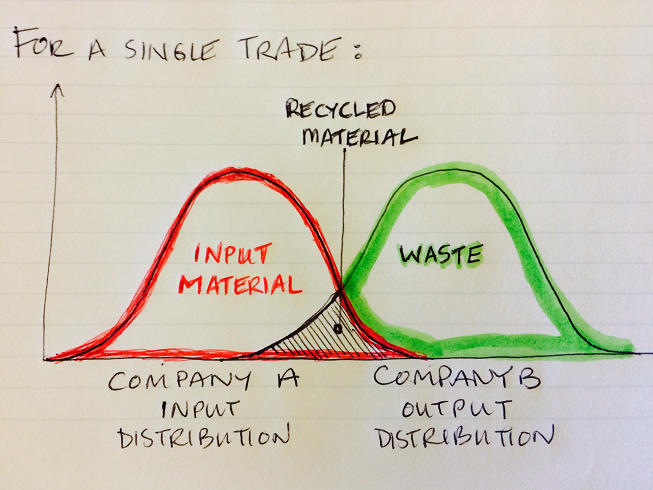
\includegraphics[width=0.5\textwidth]{figures/Variables.png}
\caption{\label{fig:Variables}Variables used in calculation of indicators, as determined for one trade between companies (redraw for final paper). Total material input, $IM$, is the sum of input material for all companies; total recycled materials, $RM$, is the sum of recycled material for all companies; the total waste, $W$, is the sum of waste for all companies.}
\end{figure}


In their study, Haas et al. (2015) estimate these indicators for the global and European economies. The authors found that the total processed materials in the global economy is 62 Gt/year (58 Gt/year raw material plus 4 Gt/year recycled), and the degree of circularity is 6 percent. The European Union was found to have 7.7 Gt/year of total processed materials with a degree of circularity of 13 percent. Waste throughput for both economies was found to be 66 percent. These real-economy values provide a point of comparison for the model results.

 
 
 
\paragraph{Geographical setup}

The initial position of companies can be setup in many ways. The most basic case is a spatial uniform distribution of coordinates, and the model is first tested on it. A more refined spatialization can be done given a population density field $d(\vec{x})$. Assuming a local scaling of companies number as a function of population of a city $N$ (not verified at a small scale, but more reasonable at a macroscopic scale), $Y \sim N^{\alpha}$, we take the probability for a firm to locate in a patch as a function of its population $\mathbb{P}\left(\vec{x}_i=\vec{x}|i\right) \propto \left(\frac{N(\vec{x}}{\sum N}\right)^{\alpha}$. Companies are thus located sequentially at random, given these probability. Population distribution can be synthetically generated, as a kernel mixture $P(\vec{x}) = \sum_{1\leq j\leq p} K_j (\vec{x})$ with $p$ number of cities (or ``centers''), and kernels $K_j(\vec{x}) = \cdot \exp{-\frac{||\vec{x}-\vec{x}_j||}{r_0}}$ where $x_j$ is random with uniform distribution and $r_0$ is computed such that the city system respects Zipf rank-size law with exponent $\gamma$ (similar values at origin assume a constant maximal center density across cities), i.e. such that $P_j = \iint K_j \propto \frac{1}{j^{\gamma}}$. For real system, we use the raster population density with 1km resolution from CIESIN~\cite{gridded2005density}.


%%%%%%%%%%%%%%%%%%
\begin{figure}
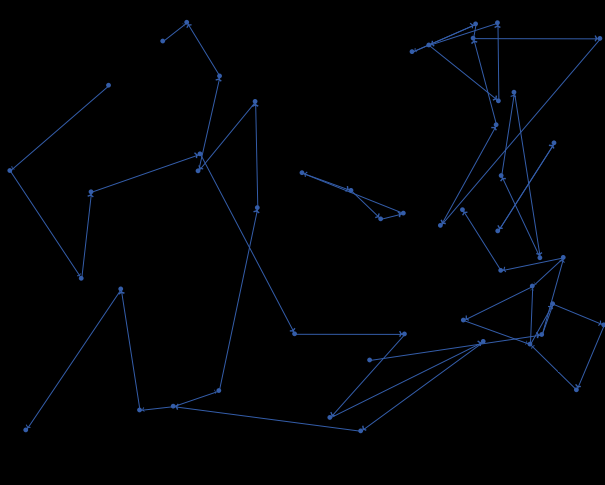
\includegraphics[width=0.32\textwidth]{figures/ex_uniform_0}
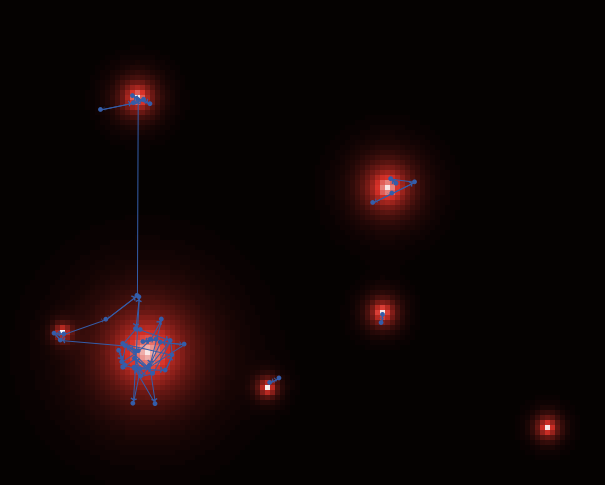
\includegraphics[width=0.32\textwidth]{figures/ex_synthetic_0}
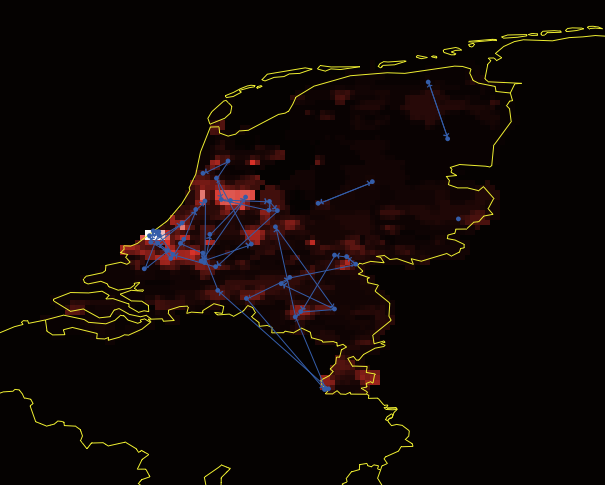
\includegraphics[width=0.32\textwidth]{figures/ex_geo_0}
\caption{Examples for three possible geographical setups (from left to right, uniform, synthetic city system, real density data)}
\label{fig:spatialization-example}
\end{figure}
%%%%%%%%%%%%%%%%%%



%%%%%%%%%%%%%%%%%%
\subsection{Extensions}

Various possible model extensions include for example :
\begin{itemize}
\item Bargain games with more than two players, implying game-theory framework to establish links among potential partners
\item Random Utility Models
\end{itemize}




%%%%%%%%%%%%%%%
% RQ : same price for each material (can be tricked with general cost)
% RQ : synthetic city generation : companies scales with P -> E ~ 1/ i ^ alpha*beta
% RQ : multiple links at time.
% RQ : maybe not that good for the other ? -> here put a proba or Game Theory ? ?

% WHEN DO WE STOP ?

% RQ : input from external ?









%%%%%%%%%%%%%%%%%%
\section{Results}

% TODO : when all line up, should be perfectly circular - sensitivity of moving slightly distribs.

% calibration on a given parc

% web application ?



%%%%%%%%%%%%%%%%%%
\subsection{Implementation}

A first prototype was implemented in \texttt{NetLogo}. Further developments will include a \texttt{R} version, especially for the integration into a \texttt{shiny} web application for a real world use as described before. Model exploration was done using model exploration software OpenMole~\cite{reuillon2013openmole}. Code and results are available on the open repository of the project\footnote{at \texttt{https://github.com/SFICSSS16-CircularEconomy/CircularEconomy}}.


%%%%%%%%%%%%%%%%%%
\subsection{Model Exploration}

%%%%%%%%%%%%%%%%%%
\subsubsection{Internal model validation}

First of all, we verify the internal consistence of the model by looking at statistical distribution of indicators (shown in fig.~\ref{fig:stat-distrib} for some points of the parameter space). Distribution are unimodal but not necessarily normal. We can however roughly estimate the number of runs needed to reach a certain confidence interval on the mean. For example, assuming normal laws, to have a $\alpha$ level CI of width $\sigma$ around the mean, the result is independent of distributions and verifies $\sigma = \frac{4\sigma \cdot z_{1-\alpha}}{\sqrt{n}}$, what gives $n\simeq 64$. We run experiments with $n=50$ in the following.


%%%%%%%%%%%%%%%%%%
\subsubsection{Uniform spatialization}

We ran first experiments with a uniform initial distribution. Figures~\ref{fig:heatmap} and~\ref{fig:pareto} show heatmaps and Pareto front.





%%%%%%%%%%%%%%%%%%
\begin{figure}
\hspace{-2cm}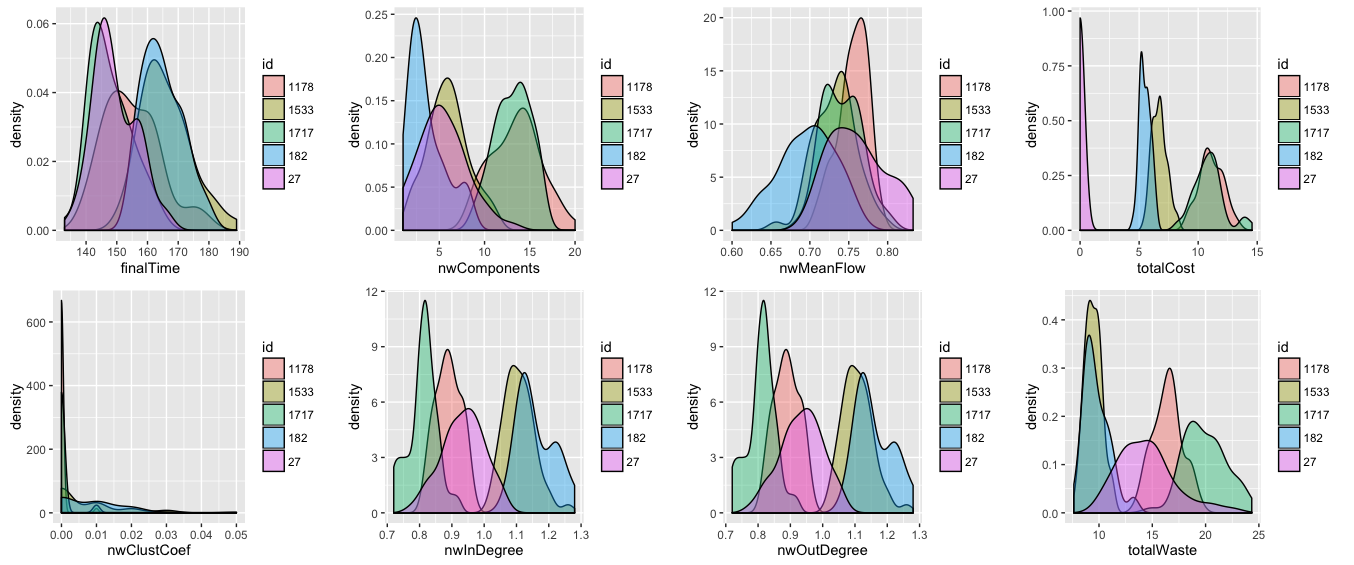
\includegraphics[width=1.3\textwidth]{figures/indics_distrib.png}
\caption{Statistical distribution of indicators for some points in the parameter space.}
\label{fig:stat-distrib}
\end{figure}
%%%%%%%%%%%%%%%%%%

%%%%%%%%%%%%%%%%%%
\begin{figure}
\hspace{-2cm}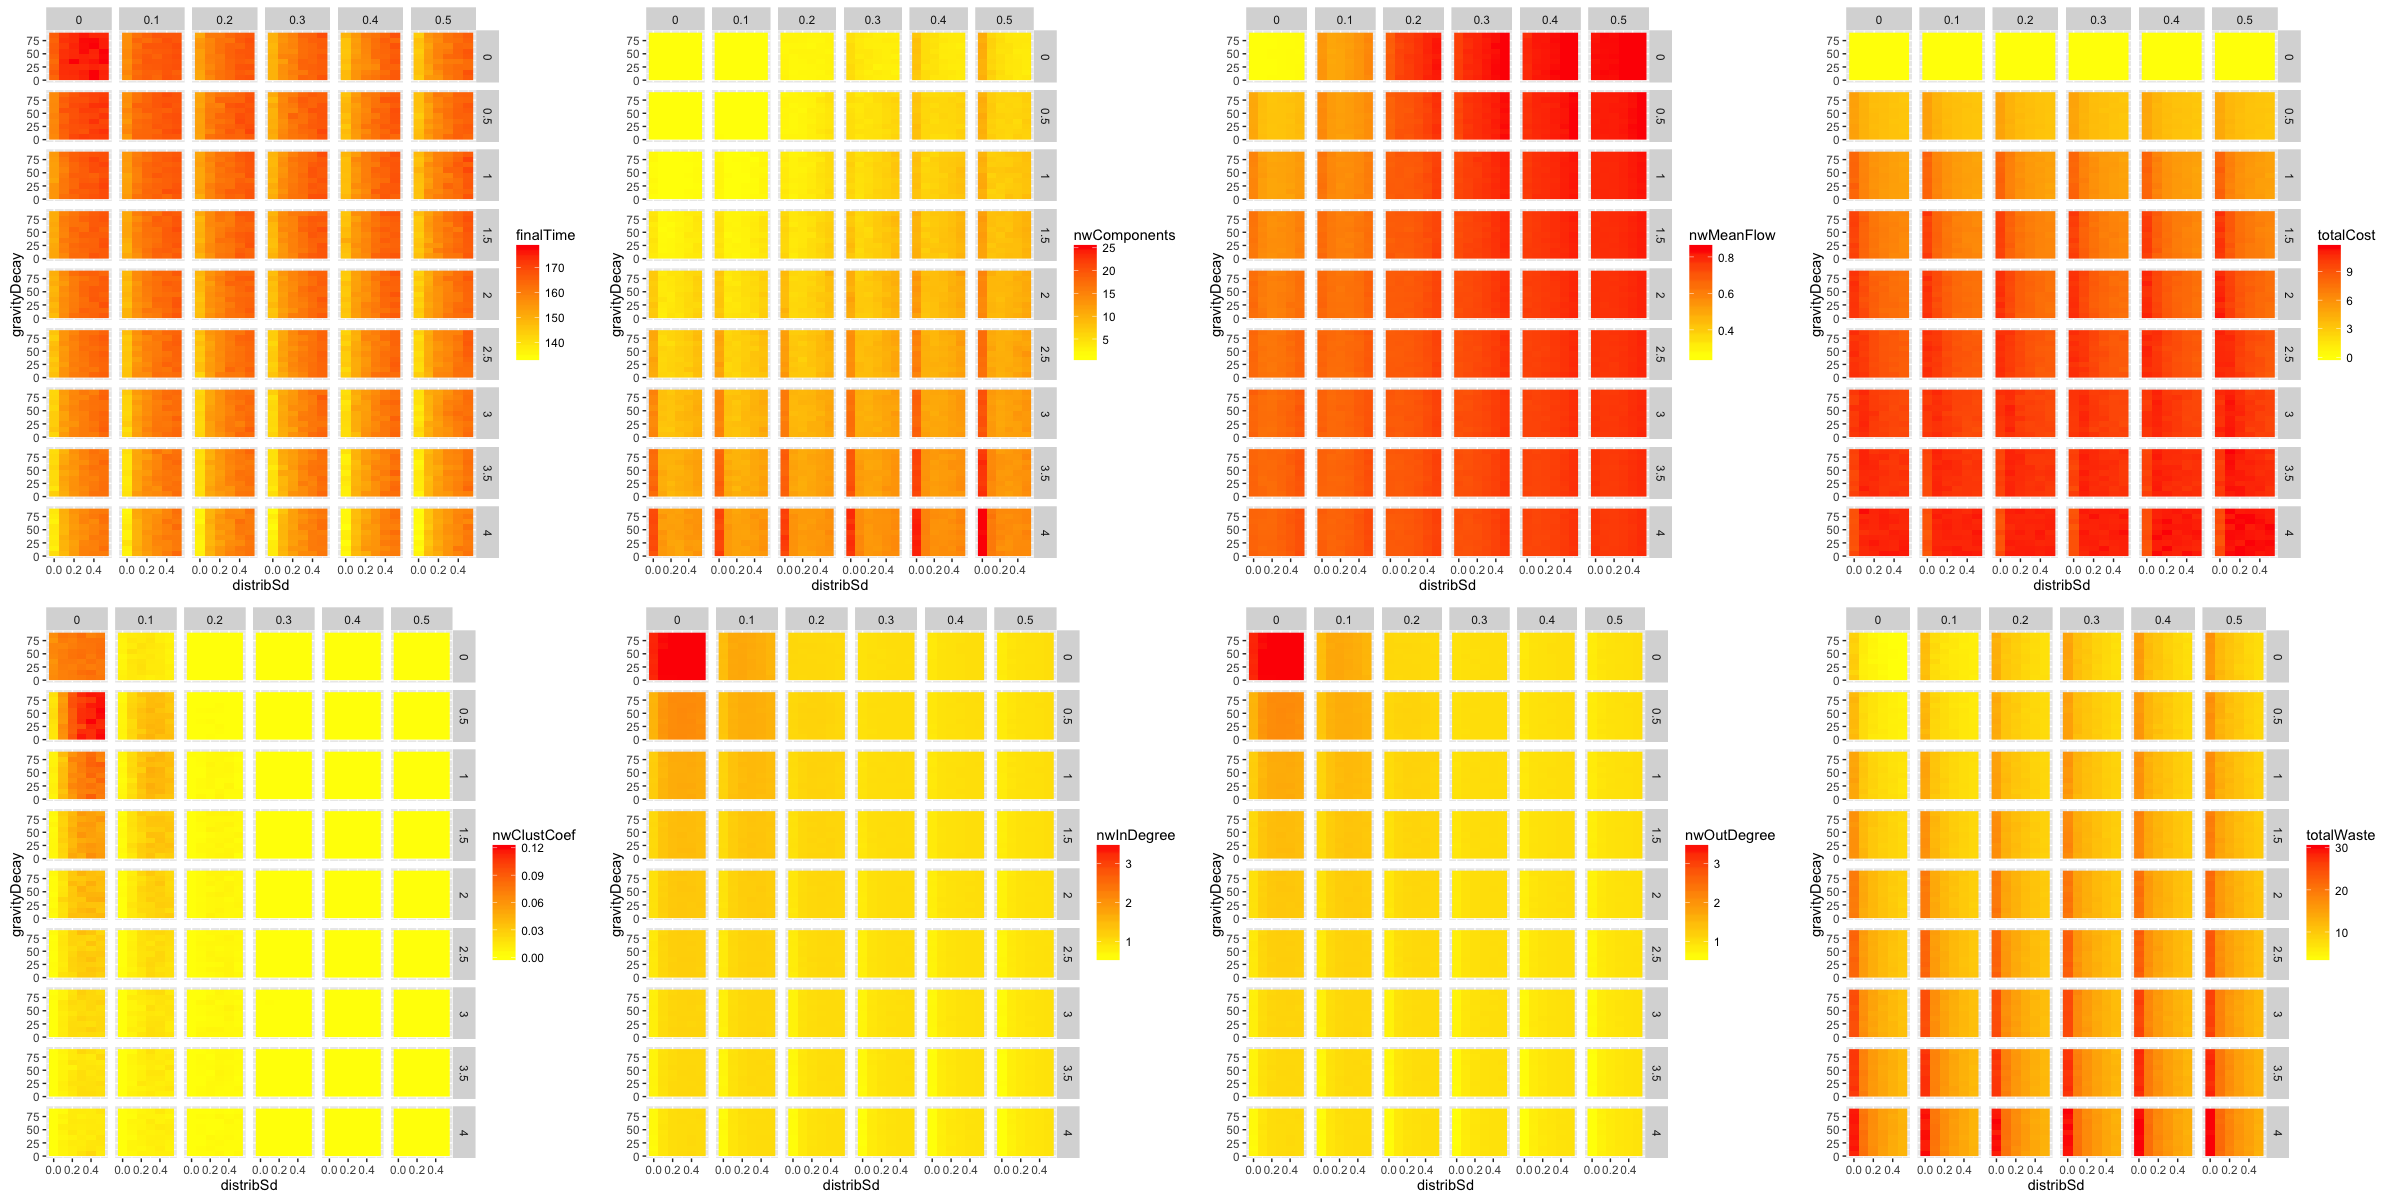
\includegraphics[width=1.3\textwidth]{figures/heatmap_indics}
\caption{Heatmaps of indicator values in the 4-D parameter space}
\label{fig:heatmap}
\end{figure}
%%%%%%%%%%%%%%%%%%

%%%%%%%%%%%%%%%%%%
\begin{figure}
\hspace{-2cm}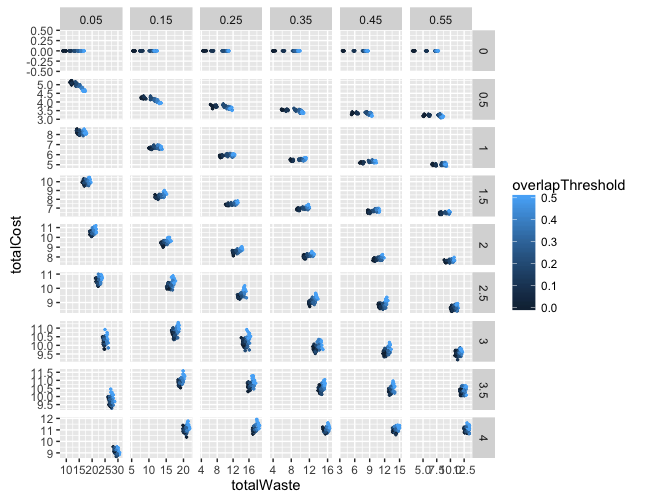
\includegraphics[width=1.3\textwidth]{figures/pareto_wasteCost_overlapThreshold}
\caption{Pareto fronts of total waste against total cost, at fixed values of transportation cost and distribution standard deviation.}
\label{fig:pareto}
\end{figure}
%%%%%%%%%%%%%%%%%%



%%%%%%%%%%%%%%%%%%
\subsubsection{Synthetic city system}

\textit{See repository for figures for similar experiments with synthetic system}

%%%%%%%%%%%%%%%%%%
\subsubsection{Real city system}

\textit{idem}

\textbf{Interesting result} : qualitative transition when changing from uniform to real system - implications for decision making ; importance to embed in a real urban system.


%%%%%%%%%%%%%%%%%%
%\begin{figure}
%\hspace{-2cm}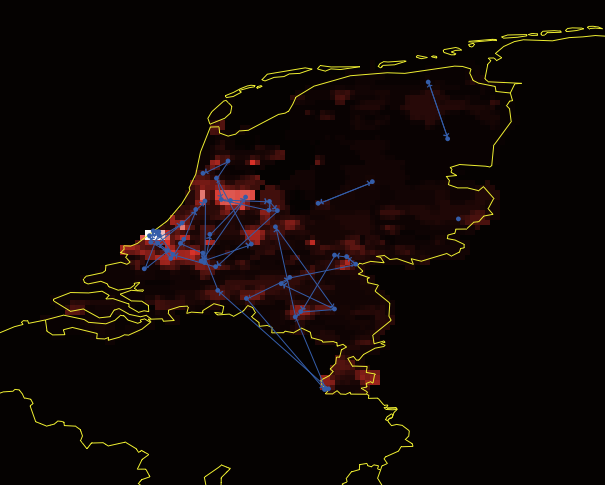
\includegraphics[width=1.3\textwidth]{figures/ex_geo_0}
%\caption{Implementation on a real city system with Netherlands}
%\label{fig:geo-example}
%\end{figure}
%%%%%%%%%%%%%%%%%%











%%%%%%%%%%%%
% biblio

%\newpage

%\bibliographystyle{apalike}
\bibliography{biblio}





\end{document}









%%%%%%%%%%%%%%%%%%%%%%%%%%%%%%%
%% TEMPLATES



%\section*{Introduction}

%The Introduction section, of referenced text\cite{Figueredo:2009dg} expands on the background of the work (some overlap with the Abstract is acceptable). The introduction should not include subheadings.

%\section*{Results}

%Up to three levels of \textbf{subheading} are permitted. Subheadings should not be numbered.

%\subsection*{Subsection}

%Example text under a subsection. Bulleted lists may be used where appropriate, e.g.

%\begin{itemize}
%\item First item
%\item Second item
%\end{itemize}

%\subsubsection*{Third-level section}
 
%Topical subheadings are allowed.

%\section*{Discussion}

%The Discussion should be succinct and must not contain subheadings.

%\section*{Methods}

%Topical subheadings are allowed. Authors must ensure that their Methods section includes adequate experimental and characterization data necessary for others in the field to reproduce their work.

%\bibliography{sample}

%\noindent LaTeX formats citations and references automatically using the bibliography records in your .bib file, which you can edit via the project menu. Use the cite command for an inline citation, e.g.  \cite{Figueredo:2009dg}.

%\section*{Acknowledgements (not compulsory)}

%Acknowledgements should be brief, and should not include thanks to anonymous referees and editors, or effusive comments. Grant or contribution numbers may be acknowledged.

%\section*{Author contributions statement}

%Must include all authors, identified by initials, for example:
%A.A. conceived the experiment(s),  A.A. and B.A. conducted the experiment(s), C.A. and D.A. analysed the results.  All authors reviewed the manuscript. 

%\section*{Additional information}

%To include, in this order: \textbf{Accession codes} (where applicable); \textbf{Competing financial interests} (mandatory statement). 

%The corresponding author is responsible for submitting a \href{http://www.nature.com/srep/policies/index.html#competing}{competing financial interests statement} on behalf of all authors of the paper. This statement must be included in the submitted article file.

%\begin{figure}[ht]
%\centering
%\includegraphics[width=\linewidth]{stream}
%\caption{Legend (350 words max). Example legend text.}
%\label{fig:stream}
%\end{figure}

%\begin{table}[ht]
%\centering
%\begin{tabular}{|l|l|l|}
%\hline
%Condition & n & p \\
%\hline
%A & 5 & 0.1 \\
%\hline
%B & 10 & 0.01 \\
%\hline
%\end{tabular}
%\caption{\label{tab:example}Legend (350 words max). Example legend text.}
%\end{table}

%Figures and tables can be referenced in LaTeX using the ref command, e.g. Figure \ref{fig:stream} and Table \ref{tab:example}.









